% =============================================================================
%  ICAIN-2026 submission — Springer LNNS / LNCS (llncs.cls) format
%  REVISED: addresses Reviewer 1 (comments 1-6) and Reviewer 2 (comments 1-7).
%
%  Requires the official Springer LaTeX2e Proceedings Templates:
%    https://www.springer.com/gp/computer-science/lncs/conference-proceedings-guidelines
%  Place llncs.cls (and splncs04.bst if you switch to BibTeX) beside this file.
%
%  FIGURES: supplied as vector PDF in figures/ (400-dpi PNG also provided),
%  regenerated by the reproduction notebook. Vector art satisfies R2 comment 1
%  at any print resolution.
% =============================================================================
\documentclass{llncs}

\usepackage[T1]{fontenc}
\usepackage{graphicx}
\usepackage{amsmath,amssymb}
\usepackage{array}
\usepackage{booktabs}
\usepackage{algorithm}
\usepackage{algpseudocode}
\usepackage{marvosym}
\usepackage{cite}
\usepackage[hidelinks]{hyperref}

\graphicspath{{figures/}}

\begin{document}

\title{A Distributed Waste Management System Using IoT, Fog Computing,
       Gossip-Based Load Balancing, and Blockchain}

% \titlerunning{A Distributed Waste Management System Using IoT and Fog Computing}

\author{Arnav Pawaskar \and
        Ahaan Mehta\,(\Letter) \and
        Chahak Daga \and
        Swarnalata Bollavarapu}

% \authorrunning{A. Pawaskar et al.}

\institute{Mukesh Patel School of Technology Management \& Engineering,\\
           SVKM's NMIMS University, Mumbai, India\\
           \email{mehtaahaan@gmail.com}}

\maketitle

% ── Abstract ──────────────────────────────────────────────────────────────────
\begin{abstract}
Rapid urbanization is increasing municipal solid waste faster than
fixed-schedule collection can handle, wasting truck-hours on empty bins while
others overflow between visits. This paper presents a coordinator-free
distributed waste management system integrating Internet of Things bin sensing,
fog-local route optimization, gossip-based inter-fog load balancing, and
blockchain auditability. Fog nodes compute routes locally without a cloud round
trip, gossip zone load with peers, and transfer bin responsibility ---
\emph{spillover} --- when a zone overloads, committing every operational event
to a permissioned hash-chained ledger. On a reproducible seeded simulation the
Nearest Neighbour (NN) router cuts travel distance by 28.1\,\% against
fixed-order collection and sits 4.53\,\% above the exact optimum; a 2-opt
refinement closes that gap to 0.82\,\% for 0.046\,ms per zone, whereas an exact
solver needs a projected 20\,s at 20 bins per zone and is unusable inside the
5\,s telemetry interval. Spillover cuts peak zone backlog from 15 to 12 bins
and load imbalance from 2.49 to 0.47 bins, degrades gracefully to 70\,\%
message loss, and keeps operating with three of five fog nodes down. Gossip
reaches all $N$ nodes in $0.93\log_2 N - 0.32$ rounds ($R^2=0.994$), and the
ledger commits in 0.027\,ms at 478.5\,B per transaction.

\keywords{Distributed Computing \and Fog Computing \and Internet of Things
\and Smart Waste Management \and Route Optimization \and Gossip Protocol
\and Blockchain \and Smart Cities}
\end{abstract}

% ── 1. Introduction ───────────────────────────────────────────────────────────
\section{Introduction}
\label{sec:intro}

Municipal solid waste is projected to rise from 2.01 billion tonnes in 2016 to
3.40 billion tonnes by 2050, fastest in South and East Asia~\cite{worldbank}.
Fixed-schedule collection ignores actual fill level: some bins are emptied
while nearly empty, wasting fuel and truck-hours, while others overflow between
visits, creating public-health and odour problems.

Three technologies close this gap. IoT sensing reports real rather than assumed
fill level. Fog computing places computation between sensors and cloud, so
decisions are taken next to the data rather than after a wide-area round
trip~\cite{bonomi,shi}. Blockchain gives municipality, contractor, and recycler
one tamper-evident record without a trusted intermediary. Each has been applied
to waste management separately; we combine them into one pipeline with no
central coordinator on the decision path.

\subsection*{Contributions}
\begin{itemize}
  \item \textbf{A coordinator-free five-layer architecture} in which every
        real-time decision is taken in the fog layer, formalized as local
        decision rules (Sect.~\ref{sec:architecture}).
  \item \textbf{A working fog runtime} in standard-library Python: NN routing,
        gossip, spillover load balancing, leader election, and a permissioned
        hash-chained ledger with quorum endorsement.
  \item \textbf{A justification of NN against stronger optimizers}, measuring
        NN, 2-opt, Or-opt, a genetic algorithm and an \emph{exact} Held--Karp
        solver on identical instances to quantify both NN's optimality gap and
        the zone size at which exact solving becomes infeasible.
  \item \textbf{A stress evaluation of gossip-based spillover} across load
        intensity, overload threshold, message loss to 70\,\%, and failure of
        up to three of five fog nodes.
  \item \textbf{A quantification of blockchain overhead} --- latency,
        throughput, storage, audit cost, energy --- against municipal demand.
  \item \textbf{A comparison with centralized cloud operation} and published
        IoT/fog systems, a sensor-inaccuracy sensitivity analysis, and an
        explicit account of the limits of simulation-only validation.
\end{itemize}

% ── 2. Related Work ───────────────────────────────────────────────────────────
\section{Related Work}
\label{sec:related}

Ten systems form the comparison set:
IoT bin monitoring (Singhvi et al.~\cite{singhvi}),
fog-plus-blockchain waste management (Damadi and Namjoo~\cite{damadi}),
blockchain chain of custody (Ahmad et al.~\cite{ahmad}), AI route
recommendation (Ghahramani et al.~\cite{ghahramani}), edge scheduling (Khanh
et al.~\cite{khanh}), a review of AI-driven systems (Nwokediegwu et
al.~\cite{nwokediegwu}), incentive-driven e-waste management with LPWAN and
edge AI (Choubey et al.~\cite{choubey}), federated-learning prediction with
blockchain logging (Palagan et al.~\cite{palagan}), CNN waste classification
(Alourani et al.~\cite{alourani}), and an AI--IoT--graph framework for
predictive collection (Anitha and Parthiban~\cite{anitha}). A recent review of
computational tools for waste management~\cite{nesmachnow} surveys the field.

Scored on the five capabilities a fielded system needs --- IoT sensing, fog
computing, route optimization, blockchain ledger, and peer-to-peer load
balancing --- each covers at most three and none covers all five; the full
matrix is reproduced by the notebook of Sect.~\ref{sec:implementation}. Two
patterns recur. Systems that optimize routes~\cite{ghahramani,anitha} or
monitor bins~\cite{singhvi} keep a central server in the loop, reintroducing
the latency and single-point-of-failure issues fog computing is meant to
avoid. Systems adopting blockchain~\cite{ahmad,palagan,damadi} treat it as an
add-on ledger rather than integrating it with real-time routing, so on-chain
records and operational decisions do not derive from one pipeline. A
meta-analysis of IoT-enabled routing~\cite{maciel} is the external reference
point for Sect.~\ref{sec:results}.

% ── 3. System Architecture ────────────────────────────────────────────────────
\section{System Architecture}
\label{sec:architecture}

Where sensors have been fitted, readings are usually forwarded to a central
server that decides what to collect, putting a wide-area round trip on the
critical path and making the fleet depend on one coordinator staying
reachable. Our architecture removes that dependency by moving every real-time
decision into the fog layer (Fig.~\ref{fig:architecture}).

\begin{figure}[htbp]
  \centering
  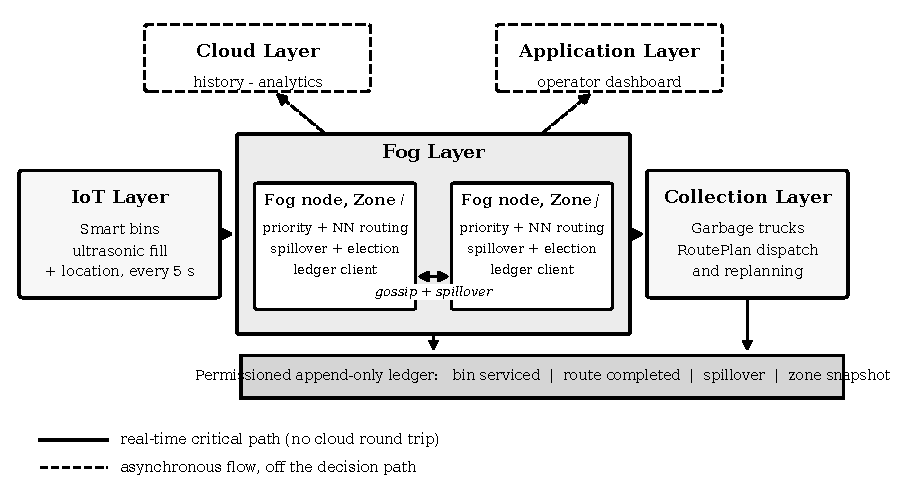
\includegraphics[width=0.93\textwidth]{fig_architecture.pdf}
  \caption{Five-layer architecture. Solid arrows mark the real-time critical
           path (bins $\rightarrow$ fog $\rightarrow$ trucks); dashed arrows
           mark asynchronous flows to the cloud and dashboard tiers, which are
           off the decision path. Fog nodes exchange zone load and transfer bin
           responsibility peer-to-peer; all operational events are committed to
           the permissioned append-only ledger.}
  \label{fig:architecture}
\end{figure}

\subsection{Formal Model}
Let $Z=\{1,\dots,N\}$ be the zones, each managed by one fog node. Zone $z$ owns
bins $B_z$; bin $b$ has position $(x_b,y_b)$ and fill level $f_b\in[0,100]$. A
bin is \emph{overflowing} when $f_b\geq\theta$ ($\theta=80\,\%$), giving the
active set and zone load
\begin{equation}
  O_z=\{\,b\in B_z : f_b \geq \theta\,\},
  \qquad n_z = |O_z| .
  \label{eq:active}
\end{equation}
Bins are ranked by a score that is total rather than merely tiered, so sorting
is deterministic:
\begin{equation}
  s(b) = 100\,w\bigl(\pi(b)\bigr) + f_b ,
  \quad
  w=\{\text{crit}\!:\!3,\ \text{high}\!:\!2,\ \text{med}\!:\!1.5,\
      \text{low}\!:\!1\},
  \label{eq:priority}
\end{equation}
where $\pi(b)$ is the tier of $b$: critical ($f_b\!\geq\!90$), high
($80\!\leq\!f_b\!<\!90$), medium ($60\!\leq\!f_b\!<\!80$), low
($f_b\!<\!60$). Only critical and high clear $\theta$ and are routed this
cycle. For depot $p_0$ and visiting order $\sigma$ of $O_z$, route cost is the
open-path Euclidean length
\begin{equation}
  D(\sigma)=\sum_{i=1}^{|O_z|}
      \bigl\lVert\, p_{\sigma(i)} - p_{\sigma(i-1)} \,\bigr\rVert_2 .
  \label{eq:routecost}
\end{equation}
The fog node minimizes~\eqref{eq:routecost} greedily, repeatedly visiting the
nearest unvisited bin. For a metric instance on $n$ nodes this is bounded
relative to the optimal tour $D^{\star}$ by~\cite{rosenkrantz}
\begin{equation}
  D_{\mathrm{NN}}/D^{\star}
  \;\leq\; \tfrac{1}{2}\bigl(\lceil \log_2 n \rceil + 1\bigr),
  \label{eq:nnbound}
\end{equation}
so the worst case degrades only logarithmically in zone size;
Sect.~\ref{sec:routing} measures the gap actually incurred.

\subsection{Layer Responsibilities}
\textbf{IoT.} Bins report \texttt{BinTelemetry} (ID, zone, $(x,y)$, fill,
timestamp) every 5\,s, fill measured by an ultrasonic sensor as a percentage of
capacity. Gas sensing is designed for but not exercised. \textbf{Fog.} Each
zone runs an independent node with a local processing unit aggregating a
\texttt{ZoneState}, a route optimizer, an inter-fog module (discovery, gossip,
spillover, election), and a ledger client; all collection decisions are taken
here. \textbf{Cloud.} Nodes asynchronously upload snapshots and
ledger-verified logs for long-term analytics; this tier is specified but not
implemented and has no real-time role. \textbf{Collection.}
\texttt{RoutePlan} objects go directly from fog nodes to trucks, with
replanning pushed mid-cycle. \textbf{Application.} A web dashboard shows fill
maps, routes, topology, election state, ledger status, and spillover logs.

% ── 4. Implementation ─────────────────────────────────────────────────────────
\section{Implementation}
\label{sec:implementation}

The fog runtime is Python (3.7+) using only standard-library modules, so it
runs on inexpensive edge hardware. Source is organized into \texttt{modules/}
(routing, inter-fog communication, election), \texttt{simulation/},
\texttt{contracts/} (data structures and ledger), and \texttt{tests/}. The
implementation, a notebook reproducing every measurement reported in
Sect.~\ref{sec:results}, and the \texttt{experiments/} scripts that render the
figures from them are at
\url{https://github.com/arnav-pawaskar/WasteManagmentSystem}.

\textbf{Route optimization.} Routing one truck around $O_z$ is a restricted
Traveling Salesman Problem. Because routes must be recomputed within the
telemetry interval whenever a bin overflows, the runtime applies the NN
heuristic of~\eqref{eq:nnbound} over priority-sorted bins;
Sect.~\ref{sec:routing} tests that choice against 2-opt~\cite{croes}, Or-opt
relocation, a genetic algorithm, and the exact Held--Karp dynamic
program~\cite{heldkarp}. When a bin not in any active route crosses $\theta$,
the processing unit interrupts the route manager, which recomputes and pushes a
revised \texttt{RoutePlan}.

\textbf{Peer discovery and gossip.} Each node announces itself to its
configured roster, tracks liveness by heartbeats refreshed from inbound gossip,
drops silent peers after a timeout, and readmits them when traffic resumes. It
periodically pushes its \texttt{ZoneState} to a random subset of peers of
bounded fanout $\phi$ (default 3) --- the rumour-mongering variant of the
epidemic protocols of Demers et al.~\cite{demers}, whose rounds to reach all
$N$ participants is $\Theta(\log N)$; Sect.~\ref{sec:spillover} measures the
constant.

\textbf{Spillover.} When the zone load $n_z$ of~\eqref{eq:active} exceeds
$\tau$ (default 10), the node ranks peers by gossip-reported load and requests
a transfer from the least loaded (Algorithm~\ref{alg:spillover}), shedding the
bins ranked lowest by~\eqref{eq:priority}. Bins moved to peer $j$ number
\begin{equation}
  \Delta_{z\rightarrow j}
  = \min\bigl(\,n_z-\tau,\ \tau-n_j,\ |O_z|\,\bigr),
  \label{eq:spill}
\end{equation}
so a receiver is never pushed past $\tau$ \emph{at the moment of transfer}.
This is a point-in-time admission test: it bounds the receiver's load on
acceptance but not its subsequent organic fill --- a distinction
Sect.~\ref{sec:spillover} quantifies. An invitation-based
election~\cite{garciamolina} designates one node to arbitrate cross-zone
conflicts; followers keep operating locally, so there is no interruption.

\begin{algorithm}[htbp]
\caption{Spillover Load Balancing}
\label{alg:spillover}
\begin{algorithmic}[1]
\Require Local zone $z$, load $n_z$, threshold $\tau$, gossip view $G$
\State \textbf{if} $n_z \le \tau$ \textbf{then return}
\State $P \leftarrow \text{sort}\bigl(\{j \in G : n_j \le \tau\},\;
       \text{key}=n_j\bigr)$
\For{each peer $j \in P$ not yet tried this episode}
  \State $\Delta \leftarrow \min(n_z-\tau,\ \tau-n_j,\ |O_z|)$
    \Comment{Eq.~\eqref{eq:spill}}
  \State send \textsc{SpilloverRequest}$(z,\Delta)$ to $j$
  \If{$j$ replies \textsc{Accept}}
    \State transfer the $\Delta$ lowest-priority bins to $j$;
           commit to ledger; \textbf{break}
  \EndIf
\EndFor
\end{algorithmic}
\end{algorithm}

\textbf{Ledger.} Bin service confirmations, route completions, spillover
transfers, and zone snapshots are committed to a permissioned append-only
ledger. Each transaction encodes event type, zone ID, timestamp, and a SHA-256
payload hash, authenticated by the committing node. Transactions are batched
into blocks carrying a Merkle root and a hash link to the predecessor; a block
is appended only after quorum endorsement by a fixed validator set. A
permissioned setting suits participants known in advance, allowing
Byzantine-fault-tolerant agreement~\cite{castro} with quorum
\begin{equation}
  q = 2f+1 \ \text{ of }\ n = 3f+1
  \quad\Longrightarrow\quad
  f = \lfloor (n-1)/3 \rfloor .
  \label{eq:quorum}
\end{equation}
At the three-zone default $f=0$: tolerating one Byzantine fault needs at least
four validators, so Sect.~\ref{sec:ledger} benchmarks from $n=4$ upward.

% ── 5. Results and Discussion ─────────────────────────────────────────────────
\section{Results and Discussion}
\label{sec:results}

\subsection{Experimental Setup}
\label{sec:setup}
All results come from a seeded, reproducible simulation; every number is
regenerated by the notebook of Sect.~\ref{sec:implementation}.
Table~\ref{tab:config} gives the full environment, bin model, and parameter
ranges. Bins are scattered uniformly over a $100\times100$ unit service area,
and fill advances each interval by $\mathcal{U}(1,5)$ percentage points plus a
burst of $\mathcal{U}(10,20)$ points with probability 0.08. A ``hot zone''
scenario multiplies one zone's fill rate by $h$ to create the imbalance
spillover must handle. Distances, optimality gaps, storage, and load-balancing
outcomes are deterministic under the fixed seeds and reproduce exactly.
Timings are wall-clock, hardware-dependent, and vary by a few percent between
runs; all quoted latencies come from one run on the machine in
Table~\ref{tab:config}, which should be cited alongside them.

\begin{table}[htbp]
\centering
\caption{Simulation environment, bin model, and parameters.}
\label{tab:config}
\footnotesize
\renewcommand{\arraystretch}{1.05}
\setlength{\tabcolsep}{3.5pt}
\begin{tabular}{llc@{\hspace{10pt}}llc}
\toprule
\textbf{Group} & \textbf{Parameter} & \textbf{Default / range} &
\textbf{Group} & \textbf{Parameter} & \textbf{Default / range}\\
\midrule
Platform & CPU        & Ryzen 9 8945H   & Bin & Telemetry interval & 5\,s \\
         & Clock      & 4.0\,GHz        &     & Initial fill  & $\mathcal{U}(10,60)\%$ \\
         & Runtime    & CPython 3.13.15 &     & Fill step     & $\mathcal{U}(1,5)$\,pp \\
         & OS         & Windows 11      &     & Burst prob.   & 0.08 \\
\cmidrule(r){1-3}
Topology & Zones      & 3 \ (3--50)     &     & Burst size    & $\mathcal{U}(10,20)$\,pp \\
         & Bins/zone  & 15 \ (10--20)   &     & Threshold $\theta$ & 80\% (70--90) \\
         & Trucks/zone& 1 \ (1--2)      &     & Sensor noise $\sigma$ & 0 (0--10\,pp) \\
         & Area       & $100\times100$  &     & Stuck rate    & 0 \ (0--0.40) \\
         & Depot      & $(50,50)$       &     &               &  \\
\cmidrule(r){4-6}
Fog      & Overload $\tau$ & 10 \ (8--14) & Ledger & Validators $n$ & 4 \ (4--16) \\
         & Fanout $\phi$   & 3            &        & Tx per block   & 8 \ (1--64) \\
         & Hot factor $h$  & 1.6 (1.0--2.4)&       &                &  \\
         & Message loss    & 0 \ (0--70\%)&        &                &  \\
         & Failed nodes    & 0 \ (0--3 of 5)&      &                &  \\
\bottomrule
\end{tabular}
\end{table}

\subsection{Route Optimization: Justifying Nearest Neighbour}
\label{sec:routing}
We compared six route builders on identical instances: the \emph{sequential}
baseline visiting bins in registration order (the fixed-schedule analogue), NN,
NN\,+\,2-opt~\cite{croes}, 2-opt\,+\,Or-opt relocation, a genetic algorithm
(population 60, 200 generations, order crossover), and exact
Held--Karp~\cite{heldkarp}. Ten runs at the default configuration give 30
zone-instances of 2--10 overflowing bins (mean 4.93), small enough that the
exact optimum was computed for \emph{every} one --- so the gaps in
Table~\ref{tab:routing} are exact, not estimated.

\begin{table}[htbp]
\centering
\caption{Route builders on 30 zone-instances (2--10 overflowing bins each).
         Gap is against the exact optimum; distance cut is system-wide against
         the sequential baseline over ten runs.}
\label{tab:routing}
\footnotesize
\renewcommand{\arraystretch}{1.05}
\setlength{\tabcolsep}{5pt}
\begin{tabular}{lrrrrr}
\toprule
\textbf{Algorithm} & \textbf{Gap} & \textbf{Worst} & \textbf{Time} &
\textbf{Max} & \textbf{Distance}\\
 & \textbf{mean (\%)} & \textbf{gap (\%)} & \textbf{mean (ms)} &
\textbf{(ms)} & \textbf{cut (\%)}\\
\midrule
Sequential (fixed order) & 43.37 & 130.36 & 0.001 & 0.001 & --- \\
Nearest Neighbour        &  4.53 &  20.93 & 0.008 & 0.025 & 28.1 \\
NN + 2-opt               &  0.82 &   8.49 & 0.046 & 0.319 & 30.5 \\
NN + 2-opt + Or-opt      &  0.34 &   5.76 & 0.128 & 0.774 & 30.9 \\
Genetic algorithm        &  1.55 &  20.93 & 101.83 & 202.73 & 30.2 \\
Exact (Held--Karp)       &  0.00 &   0.00 & 0.328 & 4.533 & 31.2 \\
\bottomrule
\end{tabular}
\end{table}

NN cuts travel distance by a mean of \textbf{28.1\,\%} (range 13.3--38.6\,\%
across runs) against fixed-order collection and lands 4.53\,\% above optimal on
average --- far inside the worst case permitted by~\eqref{eq:nnbound}, though
its worst individual zone was 20.93\,\% above optimal. NN is, however,
\emph{not} the best choice at this cost budget: adding 2-opt costs about
0.04\,ms per zone and cuts the gap to 0.82\,\%, recovering most of the
remaining distance (30.5\,\% versus 28.1\,\%). The genetic algorithm is
dominated outright --- worse than 2-opt on quality and over $2000\times$
slower.

Exact solving is tractable at these zone sizes but not beyond. Held--Karp costs
$O(n^2 2^n)$; measured medians rise from 0.05\,ms at $n=5$ to 4.34\,ms at
$n=10$ and 814\,ms at $n=16$ (Fig.~\ref{fig:routing}b), extrapolating to
roughly 20\,s at $n=20$ --- four times the entire telemetry interval. The
justification for a heuristic is therefore not that exact solving is impossible
at today's zone sizes, but that it fails abruptly as zones grow, whereas NN and
2-opt stay sub-millisecond at $n=20$ and under 35\,ms at $n=50$.
\textbf{We therefore recommend NN\,+\,2-opt as the operating configuration};
the runtime currently ships the NN builder, with 2-opt implemented and
evaluated in the notebook as a drop-in replacement.

Externally, a meta-analysis of IoT-enabled waste routing reports a pooled
distance reduction of 21.51\,\%, decomposing into 39.79\,\% across simulation
studies and 12.37\,\% across real deployments~\cite{maciel}. Our 28.1\,\% is a
simulation result and so sits \emph{below} the simulation-study average, which
we regard as conservative. A real-world pilot reports 32\,\% route-efficiency
improvement and 29\,\% lower fuel use~\cite{addas}, an IoT-assisted routing
algorithm 14\,\%~\cite{ali}.

\begin{figure}[htbp]
  \centering
  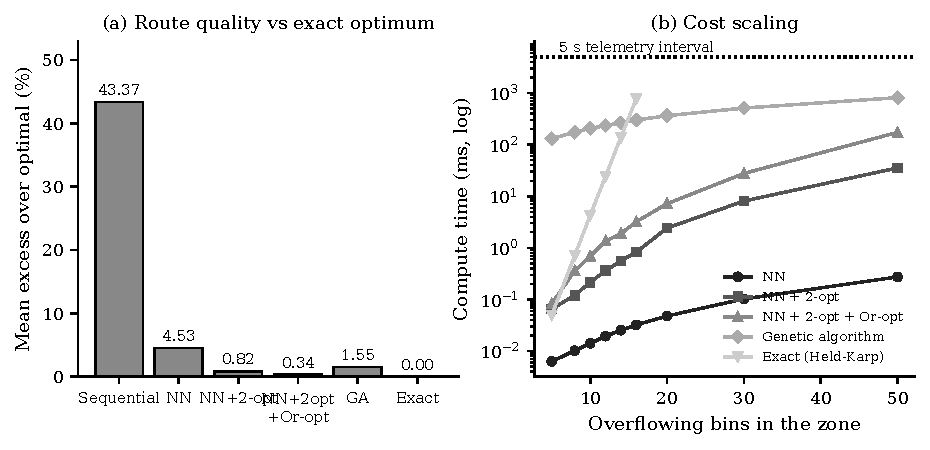
\includegraphics[width=0.93\textwidth]{fig_routing_comparison.pdf}
  \caption{(a) Mean excess over the exact optimum. (b) Compute cost against
           zone size: the exact solver crosses the 5\,s telemetry budget
           between 16 and 20 bins per zone, while the heuristics stay orders of
           magnitude below it.}
  \label{fig:routing}
\end{figure}

\subsection{Responsiveness and Scalability}
\label{sec:scale}
Injecting a new overflow into an already-routed 20-bin zone and timing
recomputation over 50 trials gives mean 0.061\,ms (median 0.061, max 0.069,
$\sigma=0.004$) --- 0.0012\,\% of the 5\,s cycle. Sweeping 3--5 zones and 10--20
bins per zone (Fig.~\ref{fig:scalability}a,b) separates two behaviours.
Per-cycle routing time grows \emph{superlinearly} in bins per zone: doubling
from 10 to 20 multiplies cycle time by 3.30--3.46$\times$, against the
2$\times$ that linear cost would predict, as expected from the $O(b^2)$ NN
construction in the number of overflowing bins $b$. The largest configuration
(5 zones, 100 bins) still completes a cycle in 0.285\,ms, or 0.0057\,\% of the
interval. Memory, measured with \texttt{tracemalloc}, grows linearly at 261\,B
per bin plus 4.39\,kB fixed overhead, spanning 12.0--30.0\,kB from 30 to 100
bins with $R^2=0.9993$ --- compatible with memory-constrained fog hardware.

\begin{figure}[htbp]
  \centering
  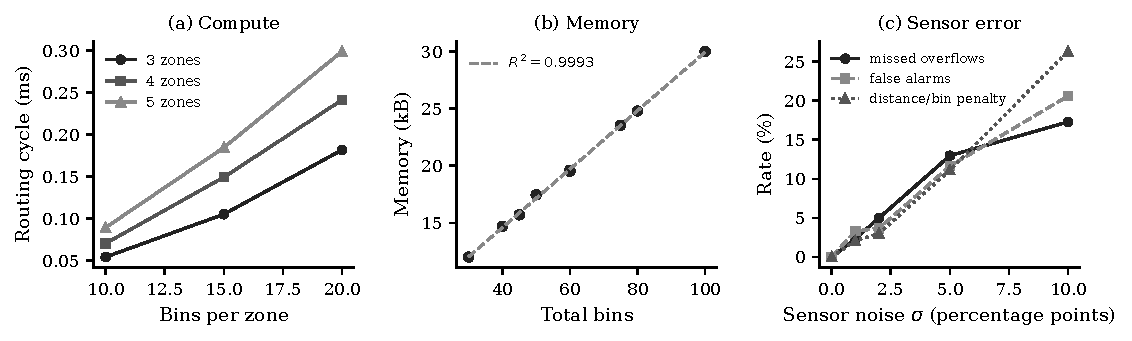
\includegraphics[width=0.93\textwidth]{fig_scalability.pdf}
  \caption{(a) Routing-cycle compute time and (b) memory footprint as zones and
           bins scale. (c) Effect of Gaussian sensor noise on overflow
           detection and on distance driven per bin serviced.}
  \label{fig:scalability}
\end{figure}

\subsection{Gossip and Spillover Under Load and Failure}
\label{sec:spillover}
We evaluated spillover along four axes (Fig.~\ref{fig:spillover}), scoring peak
zone backlog, load imbalance (standard deviation of per-zone backlog), zones
left above $\tau$, and transfers executed. Because a transfer changes which
zone owns a bin and not whether the bin is full, \emph{aggregate load is
conserved by construction}: spillover redistributes work rather than removing
it, and we report it as such.

\textbf{Load intensity.} As $h$ rises from 1.0 to 2.4, spillover consistently
removes the acute hotspot. At the default $h=1.6$ peak backlog falls from 15 to
12 bins and imbalance from 2.49 to 0.47 bins via three transfers. At mild
overload ($h=1.0$) it resolves the problem outright; under heavy overload
($h\geq1.8$) it saturates at a peak of 13, there being nowhere left to put the
bins.

\textbf{Threshold.} The point-in-time nature of~\eqref{eq:spill} shows in the
zones left above $\tau$. At $\tau=10$ spillover cuts the peak from 14.65 to
13.45 bins but still leaves 2.55 of 3 zones above threshold, because receivers
accept while compliant and then drift past $\tau$ as their own bins fill.
Raising $\tau$ to 12 leaves headroom at admission and is better on every
measure: peak 12.60, imbalance 0.53, and only 0.60 zones above threshold. The
mechanism's weakness is therefore the absence of a fill-rate forecast in the
admission decision, which a threshold tuned for headroom largely compensates.

\textbf{Message loss.} As loss rises from 0 to 70\,\%, each node's mean error
about its peers' load grows from 0 to only 1.50 bins, completed transfers fall
from 2.80 to 0.75, and peak backlog rises just 4.5\,\%, from 13.45 to 14.05
bins. Lost messages cost efficiency, not correctness: a dropped request leaves
the bins with their original owner, so none is orphaned or duplicated.

\textbf{Node failure.} With up to 3 of 5 fog nodes failed, survivors keep
balancing among themselves: peak backlog rises only from 12.75 to 13.55 bins as
transfers fall from 4.70 to 1.95. Lacking a coordinator, failures remove
capacity but never the decision-making function itself --- the property
distinguishing this design from the centralized alternative of
Sect.~\ref{sec:comparison}.

\textbf{Gossip convergence.} Over 2000 trials per configuration at $\phi=3$,
rounds for a new state to reach all $N$ nodes grow as $0.93\log_2 N - 0.32$
with $R^2=0.9936$ (1.00 rounds at $N=3$, 4.89 at $N=50$), empirically
confirming the $\Theta(\log N)$ behaviour of~\cite{demers}. At 50\,\% loss
convergence slows by about $1.6\times$ but never stalled in any trial.

\begin{figure}[htbp]
  \centering
  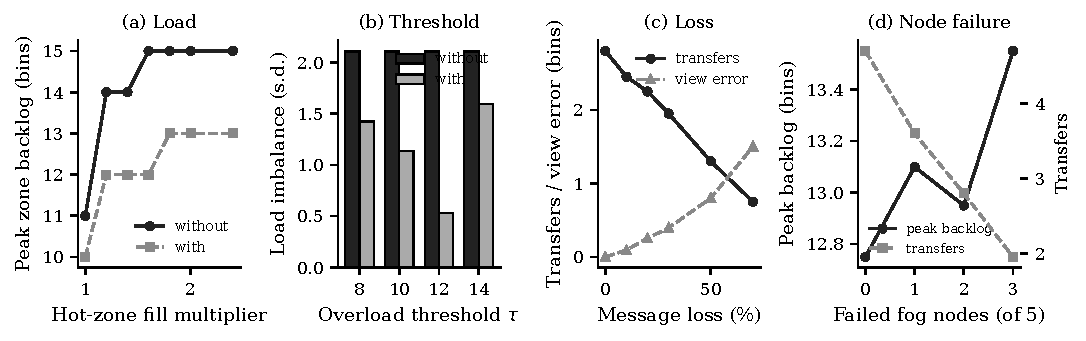
\includegraphics[width=0.93\textwidth]{fig_spillover.pdf}
  \caption{Spillover under (a) increasing hot-zone load, (b) varying overload
           threshold $\tau$, (c) message loss, and (d) fog-node failure.
           Panels (b)--(d) average 20 seeds per point.}
  \label{fig:spillover}
\end{figure}

\subsection{Blockchain Overhead}
\label{sec:ledger}
Table~\ref{tab:ledger} quantifies the cost of auditability, measured against the
ledger implementation itself rather than a stand-in.

\begin{table}[htbp]
\centering
\caption{Measured overhead of the permissioned ledger
         (4 validators, 8 transactions per block unless noted).}
\label{tab:ledger}
\footnotesize
\renewcommand{\arraystretch}{1.05}
\setlength{\tabcolsep}{5pt}
\begin{tabular}{lll}
\toprule
\textbf{Metric} & \textbf{Measured} & \textbf{Notes}\\
\midrule
Commit latency, mean     & 0.0272\,ms      & median 0.0105, p95 0.1426 \\
\quad without block seal & 0.0106\,ms      & 7 of every 8 submissions \\
\quad with block seal    & 0.1438\,ms      & propose + endorse + commit \\
Throughput               & 36\,748\,tx/s   & single-threaded, in-process \\
Seal vs.\ validators $n$ & 0.144--0.263\,ms & linear, $n=4\rightarrow16$ \\
Amortised cost per tx    & 0.0700$\rightarrow$0.0111\,ms & block size $1\rightarrow64$ \\
Storage                  & 478.5\,B/tx     & canonical JSON, marginal \\
Full-chain audit         & 15.2\,\textmu s/tx & 121.8\,ms at 8000 tx \\
Tamper detection         & detected        & payload edit fails audit \\
CPU time per tx          & 0.0286\,ms      & \texttt{process\_time} \\
Energy per tx (derived)  & 143/430/1289\,\textmu J & at 5/15/45\,W \\
\bottomrule
\end{tabular}
\end{table}

\textbf{Latency and throughput.} Cost is bimodal by design: seven of every
eight submissions merely hash, sign, and queue (0.0106\,ms), while the eighth
also seals a block (0.1438\,ms). Seal cost grows linearly with validator-set
size (0.144\,ms at $n=4$ to 0.263\,ms at $n=16$), each validator contributing
one HMAC endorsement. Batching amortises the seal: per-transaction cost falls
from 0.0700\,ms at one transaction per block to 0.0111\,ms at 64.

\textbf{Storage and audit.} The chain grows at a stable marginal 478.5\,B per
transaction, and a full independent audit --- re-checking hash linkage, block
hashes, Merkle roots, payload integrity, signatures, and endorsement quorum ---
costs 15.2\,\textmu s per transaction and scales linearly. The audit is
effective, not decorative: mutating one committed payload made
\texttt{verify\_chain} fail with the offending block and transaction
identified.

\textbf{Headroom against real demand.} A city of 100\,000 bins collected once
daily generates 1.16\,tx/s, 47.9\,MB/day and 17.5\,GB/year; at 10\,000 bins,
0.116\,tx/s and 1.75\,GB/year. Against a measured 36\,748\,tx/s the ledger has
roughly four orders of magnitude of headroom, so auditability is not the
bottleneck at municipal scale. Benchmarked Hyperledger Fabric v1.0, for
context, saturates near 140\,tx/s before optimization and about 2250\,tx/s
after~\cite{thakkar} --- even that networked figure exceeds a 100\,000-bin
city's demand by three orders of magnitude. Ours is an in-process ledger with
no network consensus, so the comparison bounds local computational cost and
claims no parity.

\textbf{Energy.} We did not instrument wall power, so we report measured CPU
time and the energy it implies through
\begin{equation}
  E_{\mathrm{op}} = P_{\mathrm{node}} \cdot t_{\mathrm{cpu}},
  \label{eq:energy}
\end{equation}
leaving $P_{\mathrm{node}}$ explicit rather than assuming a platform. At the
measured 0.0286\,ms CPU per transaction and 0.1070\,ms per three-zone routing
cycle, \eqref{eq:energy} gives 143, 430 and 1289\,\textmu J per transaction at
node powers of 5, 15 and 45\,W, and 535, 1606 and 4816\,\textmu J per cycle.
For a 10\,000-bin city committing one transaction per bin per day and running a
cycle every 5\,s, total compute energy is 10.7\,J/day at 5\,W and 96.1\,J/day
at 45\,W. Computation is thus a negligible fraction of system energy; radio
duty cycle and truck fuel dominate and are not measured here.

\subsection{Comparison with Centralized Cloud and Related Systems}
\label{sec:comparison}
\textbf{Decision latency.} Let $T_{\mathrm{dec}}$ be the time from an overflow
being observed to a revised route being available:
\begin{equation}
  T_{\mathrm{dec}} = T_{\mathrm{net}} + T_{\mathrm{comp}},
  \qquad T_{\mathrm{net}}^{\mathrm{fog}} = 0 .
  \label{eq:latency}
\end{equation}
Our measured $T_{\mathrm{comp}}$ is 0.061\,ms (Sect.~\ref{sec:scale}); a
centralized design pays $T_{\mathrm{net}}$ in addition. A large-scale
measurement study found 58\,\% of end users reach a nearby edge server in under
10\,ms but only 29\,\% achieve that latency to a nearby cloud
location~\cite{charyyev}. Substituting representative round trips
into~\eqref{eq:latency} gives 10.06\,ms via an edge server and 50.06\,ms via a
regional cloud, against 0.061\,ms fog-local --- a factor of roughly 800 at
50\,ms RTT. The network term dominates completely: this is the quantitative
case for deciding in the fog layer.

\textbf{Availability.} A centralized scheduler leaves the whole fleet unserved
when the coordinator is down, whereas coordinator-free failures are
\emph{partial}: losing $k$ of $N$ nodes leaves $N-k$ zones fully operational
rather than zero. Sect.~\ref{sec:spillover} measures this --- with 3 of 5 nodes
failed, survivors still balanced load and peak backlog rose only 6.3\,\%.
Table~\ref{tab:comparison} positions this work against the centralized
alternative and published systems.

\begin{table}[htbp]
\centering
\caption{Comparison with centralized cloud operation and representative
         IoT/fog waste-collection systems. Dashes mark capabilities the cited
         work does not address.}
\label{tab:comparison}
\footnotesize
\renewcommand{\arraystretch}{1.05}
\setlength{\tabcolsep}{4pt}
\begin{tabular}{lllllr}
\toprule
\textbf{System} & \textbf{Decision} & \textbf{Coordinator} & \textbf{Ledger} &
\textbf{P2P} & \textbf{Route}\\
 & \textbf{site} & \textbf{required} & & \textbf{balancing} & \textbf{gain}\\
\midrule
Centralized cloud (model)           & cloud  & yes & ---  & no  & --- \\
Singhvi et al.~\cite{singhvi}       & cloud  & yes & no   & no  & --- \\
Ghahramani et al.~\cite{ghahramani} & server & yes & no   & no  & yes \\
Ali et al.~\cite{ali}               & server & yes & no   & no  & 14\,\% \\
Addas et al.~\cite{addas}           & cloud  & yes & no   & no  & 32\,\%$^{\dagger}$ \\
Anitha and Parthiban~\cite{anitha}  & server & yes & no   & no  & yes \\
Damadi and Namjoo~\cite{damadi}     & fog    & yes & yes  & no  & --- \\
Palagan et al.~\cite{palagan}       & edge   & yes & yes  & no  & --- \\
Khanh et al.~\cite{khanh}           & edge   & yes & no   & yes & --- \\
\textbf{This work}                  & \textbf{fog} & \textbf{no} &
\textbf{yes} & \textbf{yes} & \textbf{28.1\,\%}\\
\bottomrule
\end{tabular}
\\[2pt]
\footnotesize $^{\dagger}$Real-world pilot; all other route gains listed are
simulation results.
\end{table}

\subsection{Sensitivity to Sensor Inaccuracy}
\label{sec:sensor}
Routing decisions use \emph{reported} fill level, so we corrupted readings and
scored the resulting decisions against ground truth
(Fig.~\ref{fig:scalability}c). With zero noise the pipeline is exact,
confirming the harness. Gaussian noise of $\sigma=1$ percentage point misses
2.33\,\% of true overflows and raises 3.32\,\% false alarms; at $\sigma=5$
these become 12.96\,\% and 11.63\,\%, and at $\sigma=10$, 17.28\,\% and
20.60\,\%, with distance per bin actually serviced rising 26.29\,\%. Stuck-at
faults, where a fouled sensor repeats its last reading, are more damaging: at a
40\,\% stuck rate 18.94\,\% of overflows are missed even at $\sigma=2$.

We also tested two standard mitigations and report a \emph{negative} result.
Exponentially-weighted moving-average smoothing ($\alpha=0.5$) and a
median-of-three filter both nearly eliminate false alarms --- from 6.31\,\% to
0.33\,\% and 0.66\,\% at $\sigma=2$ --- but both raise the miss rate roughly
\emph{fivefold}, to 27.24\,\% and 27.91\,\%. The reason is structural: bin fill
rises monotonically between collections, so any temporal filter lags the signal
and systematically under-reports. Temporal smoothing is therefore the wrong
mitigation here; redundant sensing, or threshold hysteresis biased toward early
collection, is the appropriate direction.

\subsection{Limitations and Threats to Validity}
\label{sec:limits}
\emph{Straight-line distance.} The simulation measures Euclidean, not road,
distance; real trucks follow streets, so the reported saving is optimistic.

\emph{No real-world municipal data.} The evaluation is simulation-only.
Reference~\cite{maciel} quantifies this risk precisely: pooled savings are
39.79\,\% across simulation studies but 12.37\,\% in real deployments, a factor
of about three. Our 28.1\,\% should be read as a simulation-regime figure, and
we expect materially less in the field. Validation against municipal records,
and a Raspberry Pi deployment with real ultrasonic sensors, are necessary next
steps and are not claimed here.

\emph{Prototype ledger.} Entries use HMAC-SHA256, a shared-key scheme: any
party able to verify can also forge, giving tamper evidence against outsiders
but no non-repudiation between participants. A deployment requires public-key
signatures. The agreement step is PBFT-shaped~\eqref{eq:quorum} but omits view
change and equivocation handling, and the ledger is in-process.

\emph{Unmeasured tiers and derived energy.} Leader-election latency is
implemented but not measured; gossip convergence is measured in protocol rounds
rather than seconds, so it is independent of link latency, which we do not
model. Energy is computed from measured CPU time via~\eqref{eq:energy}, not
instrumented, and excludes radio and vehicle energy. Finally, the figures
exercise the routing, replanning, spillover, gossip, and ledger paths in a
seeded harness rather than the full threaded runtime under production load.

% ── 6. Societal Impact ────────────────────────────────────────────────────────
\section{Benefits to Society}
\label{sec:society}

\textbf{Fewer truck-kilometres, less fuel and emission.} Collection transport
is the dominant operating cost and emission source in municipal waste
management. Fill-aware routing cut travel distance by 28.1\,\% in simulation,
rising to 30.5\,\% with 2-opt. Because fuel use and tailpipe emissions scale
closely with distance driven, savings of this order translate into
proportional reductions in both; a real-world pilot measured 29\,\% lower fuel
consumption from a comparable efficiency gain~\cite{addas}.

\textbf{Fewer public-health incidents.} Bins overflowing between visits create
odour, pest, and sanitation problems that fall hardest on dense, lower-income
neighbourhoods, typically served last on a fixed rota. Fill-driven
prioritization services critical bins first regardless of schedule position,
and spillover stops any zone's backlog growing without bound: peak backlog fell
from 15 to 12 bins, and inter-zone imbalance by 81\,\% at $\tau=10$. The
benefit is a more even standard of service across a city rather than a faster
average.

\textbf{Accountability between stakeholders.} Waste contracts are widely
disputed because each party keeps its own record of what was collected, when,
and by whom. The permissioned ledger gives all parties one tamper-evident
record any of them can audit independently at 15.2\,\textmu s per transaction,
without trusting an intermediary --- and a mutated record is detected
(Sect.~\ref{sec:ledger}). For a 100\,000-bin city this costs 17.5\,GB/year,
negligible against the value of settling a dispute or demonstrating regulatory
compliance.

\textbf{Affordability, and what we do not claim.} Needing only the Python
standard library, 30\,kB for 100 bins, and under 0.3\,ms per routing cycle, the
runtime fits single-board hardware costing tens of dollars per zone rather than
a metered cloud service --- relevant for the rapidly urbanizing cities where
waste growth is fastest~\cite{worldbank}. We do \emph{not} claim a validated
municipal cost saving: that requires the field deployment of
Sect.~\ref{sec:limits}.

% ── 7. Conclusion ─────────────────────────────────────────────────────────────
\section{Conclusion}
\label{sec:conclusion}

We proposed, implemented, and evaluated a distributed waste management system
unifying IoT bin monitoring, fog-local route optimization, gossip-based
coordination, spillover load balancing, and blockchain auditability, with no
central coordinator on the decision path. On a reproducible seeded simulation
the NN router cut collection distance by 28.1\,\% against fixed-order
collection while sitting 4.53\,\% above the exact optimum, and a measured
comparison against 2-opt, Or-opt, a genetic algorithm and an exact solver
showed NN\,+\,2-opt dominates at 0.82\,\% gap and 0.046\,ms. Spillover cut peak
backlog by 20\,\% and imbalance by 81\,\%, survived 70\,\% message loss and the
failure of three of five fog nodes, and proved limited by its point-in-time
admission test --- a limitation raising $\tau$ to 12 largely removes. The
ledger commits at 0.027\,ms and 478.5\,B per transaction against 1.16\,tx/s
demand from a 100\,000-bin city.

Future work follows from Sect.~\ref{sec:limits}: deployment on Raspberry Pi fog
nodes with real sensors, validated against municipal records over a road
network; promoting 2-opt into the runtime; replacing shared-key authentication
with public-key signatures and completing the Byzantine agreement path; adding
a fill-rate forecast to the spillover admission test; and incorporating
federated learning~\cite{mcmahan} to predict fill trajectories for proactive,
pre-overflow scheduling without centralizing raw telemetry.

\begin{credits}
\subsubsection{\discintname}
The authors have no competing interests to declare that are relevant to the
content of this article.
\end{credits}

% ── References ────────────────────────────────────────────────────────────────
\begin{thebibliography}{28}

\bibitem{worldbank}
Kaza, S., Yao, L.C., Bhada-Tata, P., Van Woerden, F.: What a Waste 2.0: A
Global Snapshot of Solid Waste Management to 2050. World Bank, Washington,
DC (2018)

\bibitem{bonomi}
Bonomi, F., Milito, R., Zhu, J., Addepalli, S.: Fog computing and its role in
the Internet of Things. In: Proceedings of the 1st Edition of the MCC Workshop
on Mobile Cloud Computing, pp. 13--16. Helsinki, Finland (2012)

\bibitem{shi}
Shi, W., Cao, J., Zhang, Q., Li, Y., Xu, L.: Edge computing: vision and
challenges. IEEE Internet Things J. \textbf{3}(5), 637--646 (2016)

\bibitem{singhvi}
Singhvi, R.K., Lohar, R.L., Kumar, A., Sharma, R., Sharma, L.D.,
Saraswat, R.K.: IoT based smart waste management system: India prospective.
In: Proceedings of the 4th International Conference on Internet of Things:
Smart Innovation and Usages (IoT-SIU), pp. 1--6. Ghaziabad, India (2019)

\bibitem{ahmad}
Ahmad, R.W., Salah, K., Jayaraman, R., Yaqoob, I., Omar, M.: Blockchain for
waste management in smart cities: a survey. IEEE Access \textbf{9},
131520--131541 (2021)

\bibitem{ghahramani}
Ghahramani, M., Zhou, M., Molter, A., Pilla, F.: IoT-based route
recommendation for an intelligent waste management system. IEEE Internet
Things J. \textbf{9}(14), 11883--11892 (2022)

\bibitem{khanh}
Khanh, Q.V., Nguyen, V.H., Minh, Q.N., Van, A.D., Anh, N.L., Chehri, A.: An
efficient edge computing management mechanism for sustainable smart cities.
Sustain. Comput. Inform. Syst. \textbf{38}, 100867 (2023)

\bibitem{nwokediegwu}
Nwokediegwu, Z.Q.S., Ugwuanyi, E.D., Dada, M.A., Majemite, M.T.,
Obaigbena, A.: AI-driven waste management systems: a comparative review of
innovations in the USA and Africa. Eng. Sci. Technol. J. \textbf{5}(2),
507--516 (2024)

\bibitem{choubey}
Choubey, A., Mishra, S., Misra, R., Pandey, A.K., Pandey, D.: Smart e-waste
management: a revolutionary incentive-driven IoT solution with LPWAN and
edge-AI integration for environmental sustainability. Environ. Monit. Assess.
\textbf{196}(8), 720 (2024)

\bibitem{palagan}
Palagan, C.A., Joe, S.S.A., Mary, S.J., Jijo, E.E.: Predictive
analysis-based sustainable waste management in smart cities using IoT edge
computing and blockchain technology. Comput. Ind. \textbf{166}, 104234 (2025)

\bibitem{alourani}
Alourani, A., Ashraf, M.U., Aloraini, M.: Smart waste management and
classification system using advanced IoT and AI technologies. PeerJ Comput.
Sci. \textbf{11}, e2777 (2025)

\bibitem{anitha}
Anitha, R., Parthiban, A.: AI-IoT-graph synergy for smart waste management: a
scalable framework for predictive, resilient, and sustainable urban systems.
Front. Sustain. \textbf{6}, 1675021 (2025)

\bibitem{nesmachnow}
Nesmachnow, S., Rossit, D., Moreno-Bernal, P.: A literature review of recent
advances on innovative computational tools for waste management in smart
cities. Urban Sci. \textbf{9}(1), 16 (2025)

\bibitem{damadi}
Damadi, H., Namjoo, M.: Smart waste management using blockchain. IT Prof.
\textbf{23}(4), 81--87 (2021)

\bibitem{ali}
Ali, B., Javed, M.A., Alharbi, A.A.K., Alotaibi, S., Alkhathami, M.: Internet
of Things-assisted vehicle route optimization for municipal solid waste
collection. Appl. Sci. \textbf{14}(1), 287 (2024)

\bibitem{maciel}
Maciel, R.R., Diniz de Souza, A., Almeida, R.M.A., Leite, J.P.R.R.: The
impact of IoT-enabled routing optimization on waste collection distance: a
systematic review and meta-analysis. Logistics \textbf{9}(4), 161 (2025)

\bibitem{addas}
Addas, A., Khan, M.N., Naseer, F.: Waste management 2.0 leveraging Internet
of Things for an efficient and eco-friendly smart city solution. PLOS ONE
\textbf{19}(7), e0307608 (2024)

\bibitem{rosenkrantz}
Rosenkrantz, D.J., Stearns, R.E., Lewis II, P.M.: An analysis of several
heuristics for the traveling salesman problem. SIAM J. Comput. \textbf{6}(3),
563--581 (1977)

\bibitem{croes}
Croes, G.A.: A method for solving traveling-salesman problems. Oper. Res.
\textbf{6}(6), 791--812 (1958)

\bibitem{heldkarp}
Held, M., Karp, R.M.: A dynamic programming approach to sequencing problems.
J. Soc. Ind. Appl. Math. \textbf{10}(1), 196--210 (1962)

\bibitem{demers}
Demers, A., Greene, D., Hauser, C., Irish, W., Larson, J., Shenker, S.,
Sturgis, H., Swinehart, D., Terry, D.: Epidemic algorithms for replicated
database maintenance. In: Proceedings of the 6th Annual ACM Symposium on
Principles of Distributed Computing (PODC), pp. 1--12. Vancouver, Canada (1987)

\bibitem{garciamolina}
Garcia-Molina, H.: Elections in a distributed computing system. IEEE Trans.
Comput. \textbf{C-31}(1), 48--59 (1982)

\bibitem{castro}
Castro, M., Liskov, B.: Practical Byzantine fault tolerance. In: Proceedings
of the 3rd Symposium on Operating Systems Design and Implementation (OSDI),
pp. 173--186. New Orleans, LA, USA (1999)

\bibitem{thakkar}
Thakkar, P., Nathan, S., Viswanathan, B.: Performance benchmarking and
optimizing Hyperledger Fabric blockchain platform. In: Proceedings of the
26th IEEE International Symposium on Modeling, Analysis, and Simulation of
Computer and Telecommunication Systems (MASCOTS), pp. 264--276. Milwaukee,
WI, USA (2018)

\bibitem{charyyev}
Charyyev, B., Arslan, E., Gunes, M.H.: Latency comparison of cloud datacenters
and edge servers. In: GLOBECOM 2020 --- 2020 IEEE Global Communications
Conference, pp. 1--6. Taipei, Taiwan (2020)

\bibitem{mcmahan}
McMahan, H.B., Moore, E., Ramage, D., Hampson, S., Ag\"{u}era y Arcas, B.:
Communication-efficient learning of deep networks from decentralized data.
In: Proceedings of the 20th International Conference on Artificial
Intelligence and Statistics (AISTATS). PMLR, vol. 54, pp. 1273--1282 (2017)

\end{thebibliography}

\end{document}
